\chapter{Microstrip Patch Antennas}

\section{Structure and Working of Microstrip Patch Antennas}

Microstrip Patch Antennas (MSPAs) are planar antennas widely used in modern wireless systems due to their low profile, ease of fabrication, and compatibility with printed circuit technologies. The basic structure consists of:

\begin{itemize}
    \item A conducting \textbf{patch} (typically rectangular or circular) on the top surface.
    \item A \textbf{dielectric substrate} in the middle.
    \item A continuous \textbf{ground plane} at the bottom.
\end{itemize}

The patch is usually made of copper or gold, and the substrate can be materials like FR4, RT Duroid, or Rogers, depending on the application frequency and desired dielectric properties.

\subsection*{Working Principle}

The patch functions as a resonant cavity where fringing fields at the edges of the patch radiate electromagnetic energy. At resonance, the patch dimensions are approximately:

\[
L \approx \frac{\lambda}{2\sqrt{\varepsilon_{\text{eff}}}}, \quad \text{and} \quad W = \frac{c}{2f}\sqrt{\frac{2}{\varepsilon_r + 1}}
\]

where:
\begin{itemize}
    \item $L$ is the effective length of the patch
    \item $W$ is the width
    \item $\varepsilon_r$ is the relative permittivity of the substrate
    \item $\varepsilon_{\text{eff}}$ is the effective dielectric constant due to fringing
    \item $c$ is the speed of light
    \item $f$ is the resonant frequency
\end{itemize}

The radiated field is primarily due to the fringing fields at the open edges of the patch. These fields act as radiating elements and form the primary mechanism for radiation in MSPAs.

\subsection*{Design Equations for Rectangular Patch Antennas}

For a rectangular patch antenna, the following expressions are used to design the patch dimensions:

\begin{align*}
W &= \frac{c}{2f} \sqrt{\frac{2}{\varepsilon_r + 1}} \\
\varepsilon_{eff} &= \frac{\varepsilon_r + 1}{2} + \frac{\varepsilon_r - 1}{2} \left(1 + 12 \frac{h}{W}\right)^{-1/2} \\
\Delta L &= 0.412 h \frac{(\varepsilon_{eff}+0.3)(W/h + 0.264)}{(\varepsilon_{eff}-0.258)(W/h + 0.8)} \\
L &= \frac{c}{2f \sqrt{\varepsilon_{eff}}} - 2\Delta L
\end{align*}

where:
\begin{itemize}
    \item $W$ = width of the patch
    \item $L$ = physical length of the patch
    \item $h$ = substrate height
    \item $f$ = resonant frequency
    \item $\varepsilon_r$ = relative permittivity of the substrate
    \item $\varepsilon_{eff}$ = effective dielectric constant
    \item $\Delta L$ = extension in length due to fringing
    \item $c$ = speed of light in vacuum
\end{itemize}

These equations help accurately model and fabricate MSPAs with desired resonant behavior.

\begin{figure}[H]
    \centering
    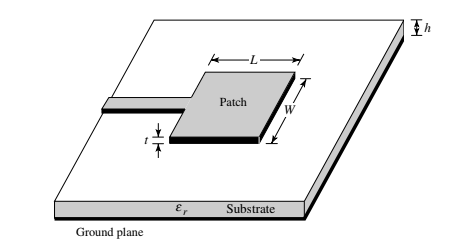
\includegraphics[width=1.0\textwidth]{figures/mspa_no_inset.png}
    \caption{Basic structure of a rectangular microstrip patch antenna (without inset feed).}
    \small Image adapted from \cite{balanis}.
    \label{fig:basic-mspa}
\end{figure}

\section{Feeding Techniques for Microstrip Patch Antennas}

There are several methods for feeding MSPAs, each with its own benefits and limitations:

\begin{itemize}
    \item \textbf{Microstrip Line Feed}: A simple and direct method, where a microstrip line is connected to the edge of the patch.
    \item \textbf{Inset Feed}: The microstrip line is inserted into the patch for impedance matching.
    \item \textbf{Coaxial Probe Feed}: A vertical coaxial probe connects the ground plane to the patch.
    \item \textbf{Aperture Coupled Feed}: Uses a slot in the ground plane to couple energy from a microstrip line below the substrate.
    \item \textbf{Proximity Coupled Feed}: Employs electromagnetic coupling between the feed line and the patch through overlapping substrates.
\end{itemize}

\subsection*{Inset Feeding}

Inset feeding is a modified microstrip line feed technique where the feed line is extended into the patch by a small distance, known as the \textit{inset distance}.

\begin{figure}[H]
    \centering
    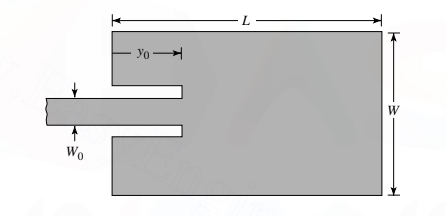
\includegraphics[width=1.0\textwidth]{figures/inset.png}
    \caption{Inset-fed rectangular microstrip patch antenna.}
    \small Image adapted from \cite{balanis}.
    \label{fig:inset-feed}
\end{figure}

\subsection*{Why Inset Feeding is Used}

The primary reason for inset feeding is to achieve \textbf{impedance matching} between the feed line (usually 50~$\Omega$) and the patch antenna, whose input impedance varies depending on the feed point location.

\begin{itemize}
    \item At the \textbf{edge of the patch}, the input impedance is high (typically 200–300~$\Omega$).
    \item By \textbf{moving the feed inward}, we reduce the input impedance to match the feed line.
    \item The \textbf{inset depth} is selected such that:
\end{itemize}

\[
Z_{\text{in}}(y_0) = Z_0 = 50~\Omega
\]

where $Z_{\text{in}}(y_0)$ is the input impedance at inset distance $y_0$, and $Z_0$ is the characteristic impedance of the microstrip line.

Inset feeding also helps maintain symmetry and reduces cross-polarization components, making it suitable for planar array applications.

\section*{Conclusion}

We have now understood the construction and operation of microstrip patch antennas, including detailed equations governing their geometry and resonance. Various feeding techniques were discussed, with inset feeding highlighted for impedance matching. This foundational knowledge will be used in the next chapter, where we simulate MSPAs under practical conditions with and without radome enclosures using ANSYS HFSS.
